%
% $Id: $
%

%\documentclass[times,10pt,twocolumn]{article}
%\documentclass[times,12pt]{article}
\documentclass[a4paper,11pt]{article}
\usepackage[utf8]{inputenc}
\usepackage{times}


\newcommand{\finejercicio}{
  \begin{footnotesize}
    [Al terminar el ejercicio es recomendable hacer \texttt{commit} de los ficheros modificados]
  \end{footnotesize}
}

\newcommand{\finpractica}{
  \begin{footnotesize}
    [Al terminar la práctica, realiza un \texttt{push} para sincronizar tu repositorio GitLab]
  \end{footnotesize}
}

%\documentstyle[times,art12,format/latex8]{article}

\usepackage{url}

\usepackage{fullpage}
\usepackage{subfigure}
\usepackage{amssymb}
\usepackage{amsmath}
\usepackage{psfrag}
\usepackage{epsfig}
\usepackage{graphicx}
\usepackage{graphics}

% COMMENTS (optional argument is author of comment)
\newcommand{\comments}[2][?]{
  \begin{quote}
    \textbf{Comment (#1):} {\em #2}
  \end{quote}
  }
%% Uncomment this line to remove comments
%\renewcommand{\comments}[2][?]{}


%-------------------------------------------------------------------------
% take the % away on next line to produce the final camera-ready version
\pagestyle{empty}

%-------------------------------------------------------------------------
\begin{document}


\title{Práctica 6 - Sesión SIP \emph{peer-to-peer}}
\author{Protocolos para la Transmisión de Audio y Vídeo en Internet}
\date{Versión 11.0.3 -- 16.12.2020}

%\author{Gregorio Robles y Jesús M. González Barahona \\
%  grex@gsyc.urjc.es \\
%  Grupo de Sistemas y Comunicaciones \\
%  Universidad Rey Juan Carlos
%}

%\date{Febrero 2010}

\maketitle
\thispagestyle{empty}

%\maketitle
%\tableofcontents
%\newpage

%-------------------------------------------------------------------------

Nota: Esta práctica se puede entregar para su evaluación como parte de la nota de prácticas, pudiendo obtener el estudiante hasta 0,7 puntos. Para las instrucciones de entrega, mira al final del documento.

\section*{Introducción}

Esta práctica tiene como objetivo implementar dos programas Python,
de manera que se pueda realizar una sesión SIP como la que se
muestra en la siguiente figura\footnote{En la figura las respuestas SIP están en 
mayúsculas para mejorar su lectura; en tu implementación deberían seguir el 
estándar, en el que sólo la primera letra es mayúscula}:

\begin{center}
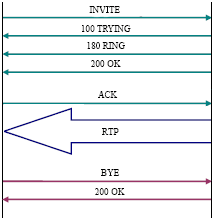
\includegraphics{figs/sip-invite.png}
\end{center}

En esta sesión:

\begin{itemize}
  \item No habrá ni servidor de registro ni \emph{proxy}. La comunicación será \emph{peer-to-peer} (directa entre dos UAs\footnote{UA: User Agent. Un UA se compone de un cliente y un servidor, aunque en esta práctica -por simplificación- cada UA tendrá sólo una de las dos partes.}).
  \item El UA de la izquierda constará exclusivamente de la parte cliente. Esta parte será la que inicie la sesión con un \texttt{INVITE} y la cierre con un \texttt{BYE}.
  \item El UA de la derecha constará exclusivamente de la parte servidora. Esta parte será la que envíe el audio vía RTP al cliente.
\end{itemize}


\section*{Objetivos de la práctica}

\begin{itemize}
  \item Implementación de una conversación de audio iniciada con SIP.
\end{itemize}

\section*{Conocimientos previos necesarios}

\begin{itemize}
  \item Nociones de SIP (las de clase de teoría)
  \item Funcionamiento de \texttt{wireshark}.
\end{itemize}

Tiempo estimado: 10 horas

\section*{Creación de repositorio para la práctica}

Con el navegador, dirígete al repositorio \texttt{ptavi-p6} en la cuenta de \emph{ptavi} en GitLab\footnote{\url{http://gitlab.etsit.urjc.es/ptavi/ptavi-p6}} y realiza un \texttt{fork}, de manera que consigas tener una copia del repositorio en tu cuenta de GitLab. Clona el repositorio que acabas de crear a local para poder editar los archivos. Trabaja a partir de ahora en ese repositorio, sincronizando los cambios que vayas realizando.

Como tarde al final de la práctica, deberás realizar un \texttt{push} para subir tus cambios a tu repositorio en GitLab. En esta práctica, al contrario que con las demás, se recomienda hacer frecuentes \texttt{commits}, pero el \texttt{push} al final.


\section*{Parte cliente}

El cliente ha de ejecutarse de la siguiente manera:
\begin{verbatim}
  $ python3 client.py metodo receptor@IPreceptor:puertoSIP
\end{verbatim}

donde \emph{metodo} será un método SIP, \texttt{receptor@IPreceptor:puertoSIP}
será el login, la IP y el puerto\footnote{En el mundo ``real'', el puerto sería 
el puerto de SIP por defecto, el 5060, ya que sólo puede haber un UA activo
por máquina - si arrancas otro UA SIP cuando hay uno ya lanzado, no te dejará.
Como en la práctica final tendremos dos UAs en la
misma máquina, hemos de especificar un puerto para que no se ``pisen''.}
al que se dirige el mensaje.

Por ejemplo:
\begin{verbatim}
  $ python3 client.py INVITE batman@193.147.73.20:5555
  $ python3 client.py BYE batman@193.147.73.20:5555
\end{verbatim}

En caso de no introducir el número de parámetros correctos o de error en los mismos, el programa debería imprimir siempre por pantalla:

\begin{verbatim}
  Usage: python3 client.py method receiver@IP:SIPport
\end{verbatim}

\subsection*{Peticiones SIP}

El cliente debería poder enviar las siguientes peticiones SIP:

  \begin{itemize}
    \item INVITE sip:receptor@IP SIP/2.0

    Mediante este método, el UA indica que quiere iniciar una conversación con el receptor con dirección \emph{receptor} en la máquina dada por la \emph{IP}\footnote{La IP puede ser 127.0.0.1.}.

    \item ACK sip:receptor@IP SIP/2.0

    Método de asentimiento. No se pasará al programa \texttt{client.py} como parámetro desde
la \texttt{shell}, ya que se enviará de manera automática una vez se hayan recibido las respuestas \texttt {100 Trying}, \texttt{180 Ring} y \texttt{200 OK} de la parte servidora.

    \item BYE sip:receptor@IP SIP/2.0

    Mediante este método se indica que queremos terminar una conversación con el receptor con dirección \emph{receptor} en la máquina dada por la IP. Se deberá enviar una vez haya acabado de recibir \emph{streaming} de audio (vía RTP) enviado desde el servidor.

  \end{itemize}


\section*{Parte servidora}

El servidor ha de ejecutarse de la siguiente manera:
\begin{verbatim}
  $ python3 server.py IP puerto fichero_audio
\end{verbatim}

Por ejemplo:
\begin{verbatim}
  $ python3 server.py 127.0.0.1 5555 cancion.mp3
\end{verbatim}

En caso de no introducir el número de parámetros correctos o de error en los mismos (se ha de comprobar si existe el fichero de audio), el programa debería imprimir:
\begin{verbatim}
  Usage: python3 server.py IP port audio_file
\end{verbatim}

En caso de no haber error al arrancar, el servidor imprimirá por pantalla:
\begin{verbatim}
  Listening...
\end{verbatim}

\subsection*{Códigos de respuesta}

   \begin{itemize}
     \item \texttt{SIP/2.0 100 Trying}: al recibir un INVITE.
     \item \texttt{SIP/2.0 180 Ringing}: al recibir un INVITE.
     \item \texttt{SIP/2.0 200 OK}: en caso de éxito.
     \item \texttt{SIP/2.0 400 Bad Request}: si la petición está mal formada.
     \item \texttt{SIP/2.0 405 Method Not Allowed}: si se manda en la petición cualquier otro método diferente de INVITE, BYE o ACK.
   \end{itemize}

Para simplificar la práctica, se enviará {\bf en un único mensaje} (i.e., un único paquete) la respuesta \texttt{SIP/2.0 100 Trying}, \texttt{SIP/2.0 180 Ringing} y \texttt{SIP/2.0 200 OK}.


\section*{Ejercicios alternativos}

Dependiendo de tu último número de tu DNI / NIE, deberás realizar los siguientes ejercicios que se describen en la Tabla~\ref{tab:ejercicios}.

\begin{center}
  \begin{table}
    \center
    \begin{tabular}{| c | c | c | c | c | c | c |} \hline
    Último número DNI/NIE & Ej. A & Ej. B & Ej. C & Ej. D & Ej. E & Ej. F \\ \hline \hline
    0 & X &   &   & X &   & X \\ \hline
    1 & X &   &   & X & X &  \\ \hline
    2 & X &   & X &   &   & X \\ \hline
    3 & X &   & X &   & X &  \\ \hline
    4 & X &   &   & X &   & X \\ \hline
    5 &   & X & X &   &   & X \\ \hline
    6 &   & X & X &   & X & \\ \hline
    7 &   & X &   & X & X & \\ \hline
    8 &   & X &   & X &   & X  \\ \hline
    9 &   & X &   & X & X &  \\ \hline
    \end{tabular}
  \caption{Tabla de ejercicios alternativos a realizar según el último número de DNI/NIE del estudiante.}
  \label{tab:ejercicios}
  \end{table}
\end{center}


\subsection*{Ejercicio A}

El cuerpo del INVITE debe incluir la descripción de sesión en formato SDP (\emph{Session Description Protocol}). Contará con los siguientes parámetros:

\begin{itemize}
  \item v (versión, por defecto la ``0''),
  \item o (origen e identificador de sesión: la dirección del origen y su IP),
  \item s (nombre de la sesión, que puede ser el que se desee),
  \item t (tiempo que la sesión lleva activa, en nuestro caso, siempre 0), y
  \item m (tipo de elemento multimedia y puerto de escucha y protocolo de transporte utilizados, en esta práctica ``audio'', el número de puerto pasado al programa principal como parámetro y ``RTP'').
\end{itemize}

Así, un ejemplo de descripción de sesión dentro de un INVITE podría ser:

\begin{verbatim}
INVITE sip:INVITE batman@193.147.73.20 SIP/2.0

v=0
o=robin@gotham.com 127.0.0.1
s=misesion
t=0
m=audio 34543 RTP
\end{verbatim}

El servidor guardará la dirección de origen y la dirección IP en un diccionario\footnote{Este diccionario ha de ser un atributo de clase no de la instancia, véase \url{http://www.toptal.com/python/python-class-attributes-an-overly-thorough-guide}} para utilizarlo posteriormente en el envío de RTP.

Nótese que en el ejemplo anterior 34543 es el puerto donde esperamos que el otro participante en la conversación nos envíe los paquetes RTP con audio. También se ha de tener en cuenta que entre las cabeceras (en este caso la línea de INVITE) y el cuerpo (la descripción de la sesión) ha de haber obligatoriamente una línea en blanco.

\subsection*{Ejercicio B}

El cuerpo de la respuesta 200 OK al INVITE debe incluir la descripción de sesión en formato SDP (\emph{Session Description Protocol}). Contará con los siguientes parámetros:

\begin{itemize}
  \item v (versión, por defecto la ``0''),
  \item o (origen e identificador de sesión: la dirección del origen y su IP),
  \item s (nombre de la sesión, que puede ser el que se desee),
  \item t (tiempo que la sesión lleva activa, en nuestro caso, siempre 0), y
  \item m (tipo de elemento multimedia y puerto de escucha y protocolo de transporte utilizados, en esta práctica ``audio'', el número de puerto pasado al programa principal como parámetro y ``RTP'').
\end{itemize}

Así, un ejemplo de descripción de sesión dentro de un INVITE podría ser:

\begin{verbatim}
SIP/2.0 200 OK

v=0
o=batman@gotham.com 127.0.0.1
s=misesion
t=0
m=audio 67876 RTP
\end{verbatim}

Se ha de tener en cuenta que entre las cabeceras (en este caso la línea de INVITE) y el cuerpo (la descripción de la sesión) ha de haber obligatoriamente una línea en blanco. Nótese que como el UA que inicia la conversación no envía paquetes RTP, la información en el SDP no se utilizará.


\subsection*{Ejercicio C}

El envío RTP se realizará mediante la biblioteca \texttt{simplertp}\footnote{En el repositorio se encuentra el módulo Python \texttt{simplertp.py}}. Un ejemplo del código Python de envío de paquetes RTP sería el siguiente:

\begin{verbatim}
  import simplertp

  RTP_header = simplertp.RtpHeader()
  RTP_header.set_header(pad_flag=0, ext_flag=0, cc=0, marker=0, ssrc=ALEAT)
  audio = simplertp.RtpPayloadMp3(audio_file)
  simplertp.send_rtp_packet(RTP_header, audio, ip, port)
\end{verbatim}

Donde ALEAT será un número entero aleatorio obtenido a partir de la biblioteca \texttt{random} de Python3\footnote{https://docs.python.org/3.8/library/random.html}.

La IP y puerto a la que se ha de enviar el RTP vendrá dada en el SDP (Ejercicio A). En el caso de que el estudiante no tenga que realizar ese ejercicio, utilizará la IP 127.0.0.1 y el puerto 23032 como destino del envío.

Nótese que \texttt{audio\_file} es uno de los parámetros que se le pasa al servidor al ejecutarse desde la línea de shell como parámetro. También ha de notarse que si sale el aviso {\bf Warning: Connection refused. Probably there is nothing listening on the other end.} es porque no hay ningún servicio \emph{escuchando} al otro lado; no es un error, indica que los paquetes han llegado al destino final, pero que no han sido gestionados.

\subsection*{Ejercicio D}

El envío RTP se realizará mediante la biblioteca \texttt{simplertp}\footnote{En el repositorio se encuentra el módulo Python \texttt{simplertp.py}}. Un ejemplo del código Python de envío de paquetes RTP sería el siguiente:

\begin{verbatim}
  import simplertp

  RTP_header = simplertp.RtpHeader()
  RTP_header.set_header(version=2, marker=BIT, payload_type=14, ssrc=200002)
  audio = simplertp.RtpPayloadMp3(audio_file)
  simplertp.send_rtp_packet(RTP_header, audio, ip, port)
\end{verbatim}

Donde BIT será un bit aleatorio obtenido a partir de la biblioteca \texttt{secrets} de Python3\footnote{https://docs.python.org/3/library/secrets.html}.

La IP y puerto a la que se ha de enviar el RTP vendrá dada en el SDP (Ejercicio A). En el caso de que el estudiante no tenga que realizar ese ejercicio, utilizará la IP 127.0.0.1 y el puerto 23032 como destino del envío.

Nótese que \texttt{audio\_file} es uno de los parámetros que se le pasa al servidor al ejecutarse desde la línea de shell como parámetro. También ha de notarse que si sale el aviso {\bf Warning: Connection refused. Probably there is nothing listening on the other end.} es porque no hay ningún servicio \emph{escuchando} al otro lado; no es un error, indica que los paquetes han llegado al destino final, pero que no han sido gestionados.


\subsection*{Ejercicio E}

Se ha de añadir la cabecera \texttt{Content-Type: application/sdp} a {\bf todos} los paquetes SIP que contengan SDP.

Así, un ejemplo de descripción de sesión dentro de un INVITE podría ser:

\begin{verbatim}
INVITE sip:INVITE batman@193.147.73.20 SIP/2.0
Content-Type: application/sdp

v=0
o=robin@gotham.com 127.0.0.1
s=misesion
t=0
m=audio 34543 RTP
\end{verbatim}


\subsection*{Ejercicio F}

Se ha de añadir la cabecera \texttt{Content-Length}, cuyo valor será la longitud (en bytes) del cuerpo del paquete, a {\bf todos} los paquetes SIP que contengan SDP.

Así, un ejemplo de descripción de sesión dentro de un INVITE podría ser:

\begin{verbatim}
INVITE sip:batman@193.147.73.20 SIP/2.0
Content-Length: 66

v=0
o=robin@gotham.com 127.0.0.1
s=misesion
t=0
m=audio 34543 RTP
\end{verbatim}




\section*{Captura}

Una vez terminada la práctica, se pide que se realice una captura de un
establecimiento de llamada, el envío RTP de audio y la finalización de
la llamada. 

La captura original se filtrará para que sólo incluya los paquetes
SIP y los tres primeros y tres últimos paquetes RTP con audio\footnote{Los heurísticos de Wireshark puede que no identifiquen los paquetes RTP como tales, sino como paquetes UDP. La solución es la siguiente: en el menú de ``Analyze'', selecciona ``Enabled protocols'' y ahí busca por RTP para activar ``rtp\_udp''.}.

La captura filtrada resultante se guardará en el fichero \texttt{invite.libpcap}
y se subirá al repositorio.


\section*{Fecha y modo de entrega}

La entrega de práctica se deberá hacer antes del miércoles 16 de diciembre de 2020 a las 23:59. Para entonces, se debe tener un repositorio \texttt{git} en GitLab con: 

    \begin{itemize}
        \item 2 módulos Python y la captura realizada con \texttt{wireshark}:
    \begin{itemize}
      \item \texttt{server.py}
      \item \texttt{client.py}
      \item \texttt{invite.libpcap}
    \end{itemize}
\end{itemize}

Se han de tener en cuenta las siguientes consideraciones:
\begin{itemize}
  \item Se valorará que al menos haya diez \emph{commits} realizados en al menos dos días diferentes.
  \item Se valorará que la captura esté bien filtrada y sólo contenga los paquetes que se indican en el guión.
  \item Se valorará que el código entregado siga la guía de estilo de Python (véanse PEP8 y PEP257).
  \item Se valorará que los programas se invoquen correctamente y que muestren los errores correctamente, según se indica en el enunciado de la práctica.
\end{itemize}

Se puede comprobar la correcta entrega de la práctica utilizando el programa \texttt{check-p6.py}. Este programa se ejecuta desde la línea de comandos de la siguiente manera:
\begin{verbatim}
  $ python3 check-p6.py login_gitlab
\end{verbatim}


donde \texttt{login\_gitlab} es tu nombre de usuario en GitLab.


%-------------------------------------------------------------------------
%\nocite{ex1,ex2}
%\bibliographystyle{format/latex8}
%\bibliography{libresoft}

\end{document}
